\chapter{Grundlagen}
\label{ch:fundamentals}

Dieses Kapitel möchte einige Grundlagen definieren, welche im Kapitel~\ref{ch:main-matter} vorausgesetzt werden.
Es handelt von der Definition des funktionalen Programmier-Paradigmas, welches in den Sprachen Clojure und Elm zum Einsatz kommt.
Weiterhin werden die Webtechnologien Websockets und \acp{SPA} erklärt, welche das Frontend des \nameref{ch:main-matter}'s nutzt. 
Die Architektur der ganzen Applikation wird maßgebend durch die Trennung in unabängige Microservices beeinflusst, welche mit Docker realisiert ist.
Als Integrationspunkt fungiert Apache Kafka, welches ebenso in diesen Kapitel erklärt wird.
\section{Funktionale Programmierung}
Die funktionale Programmierung gehört zu den Deklarativen Programmierparadigmen und stellt neben der imperativen und objektorientierten Programmierung eines der am Häufigsten genutzten Paradigmen dar.
\par
Anders als bei imperativen Sprachen, unterscheiden sich funktionale Sprachen vor Allem an ihrer Unveränderbarkeit (engl. Immutability) von Variablen und ihrer Datenstrukturen.
Es wird dabei angestrebt, bei einer Veränderung des Zustandes einer Variablen nicht den Inhalt ihrer Referenz zu verändern, sondern stattdessen eine Kopie der Daten zurückzuliefern.
In der Praxis(TODO: quote) hat sich vielfach herausgestellt, dass sich die häufig verwendete Veränderbarkeit (engl. Mutability) von Zuständen gerade auch in der objektorientierten Programmierung zu häufigen Fehlerquellen führen kann.
Es wurde jedoch gezeigt, dass das Zurückgeben von Kopien ebenso sehr performant funktionieren kann (TODO: add quote).
\par
Wie der Name schon vermuten lässt basiert die funktionale Programmierung zu größten Teilen aus Funktionen. 
Diese sind meist als Module gekapselt, welche nach einer bestimmten Aufgabe gruppiert sind. 
Anders als bei Objekten möchte man offen mit den an die Funktionen übergebenen Daten umgehen und sie nicht in der Implementierung verstecken (engl. Information-Hiding). 
Dabei sollte eine Funktion nur diese eine Aufgabe erledigen, welche mithilfe ihres Namens beschrieben wird. 
Um dieses deterministische Verhalten zu erreichen, werden oft sehr granulare Funktionen erstellt, welche anschließend durch eine Komposition miteinander vereint werden\footnote{\texttt{f(x) = g(x) • h(x) <=> f(x) = h(g(x))}}.
Jegliche Seiteneffekte sollten vermieden werden, was man auch als reine (engl. pure) Funktionen bezeichnet.
So sollten Funktionen als Daten-Transformationen verstanden werden: Man erhält Daten, verarbeitet diese und gibt sie anschließend transformiert zurück, welches als \ac{EVA}-Prinzip bekannt ist.
\par
Da Funktionen selbst auch Typen darstellen, können sie ebenso als Parameter anderer Funktionen dienen, welche man dann auch als Funktionen Höherer Ordnung (engl. Higher Order Funktions) bezeichnet.
Mit dieser Voraussetzung können Verhalten aus einer aufzurufenden Funktion heraus gelöst werden, womit das jeweilige Verhalten dynamisch bestimmt werden kann.
Dies wird oft auch als Callbacks bezeichnet.
Hilfreich sind bei dieser Vorgehensweise auch so genannte Lamdas, welche Funktionen darstellen, die inline definiert werden können und somit anonym \ac{bzw.} Unbenannt sind.
\par
Grundsätzlich werden funktionale Sprachen nochmals zwischen solchen Sprachen unterschieden, welche neben anderen Paradigmen auch das Funktionale Paradigma unterstützen und solchen, welche ausschließlich auf den Prinzipien der funktionalen Programmierung beruhen.
Die sogenannten reinen funktionalen Sprachen verbieten \ac{bspw.} eine jegliche Möglichkeit Seiteneffekte auszuführen und sind sehr oft strikt typisiert.
In Multiparadigmensprachen beruhen viele funktionale Prinzipien auf deren Einsatz und der generellen Bedachtheit des jeweiligen Programmierers \ac{bzw.} des einsetzenden Teams.

\section{Verwendete Programmiersprachen}
\subsection{Clojure}
\blindtext
\par
\blindtext
\subsection{Elm}
\blindtext
\par
\blindtext
\section{Eingesetzte Webtechnologien}
\subsection{Websockets}
\blindtext
\subsection{\aclp{SPA}}
\blindtext
\section{Microservices}
\blindtext
\section{Container-Virtualisierung mit Docker}
\begin{figure}
  \centering
  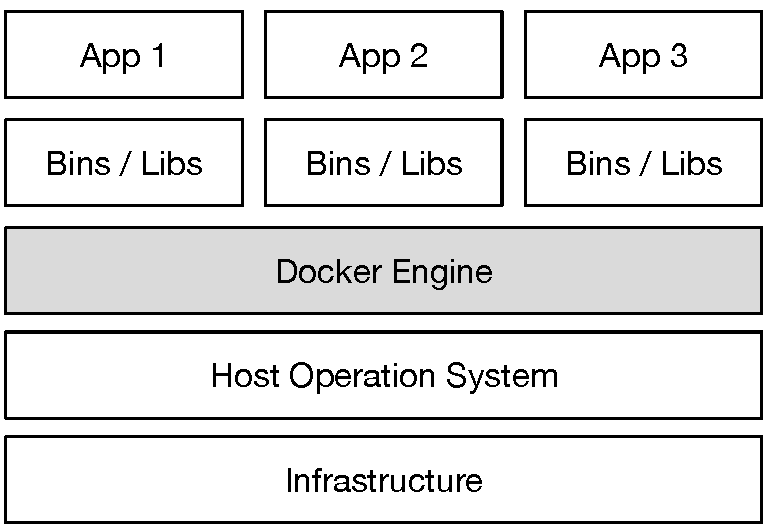
\includegraphics[scale=0.75]{docker.pdf}
  \par
  \caption{Schichten einer Virtualisierung mit Docker}
  \label{fig:layers-docker}
\end{figure}
Docker\footnote{\url{https://docs.docker.com/}} ist eine Software zum Deployment von Applikationen innerhalb von Containern.
Im Vergleich zu \acp{VM}, ähnelt sich die Vorgehensweise, jedoch laufen die Prozesse der Container direkt auf dem Host-Betriebssystem.
Trotz dieser Tatsache sind die Prozesse mithilfe von \ac{u.A.} Control-Groups und Kernel Namespaces voneinander isoliert.
Weiterhin hat man die Möglichkeit mit gängigen Mandatory-Access-Control-Frameworks wie SE-Linux oder App-Armor die Rechte innerhalb der Container zu beschränken.
Als Anforderung besteht keine spezifische Hardware-Infrastruktur wie bei beispielsweise VMWare ESXi.
Ebenso ist Docker mittlerweile auf allen gängigen Betriebssystemen lauffähig, wobei Linux-Derivate die beste Unterstützung erhalten.
Dies ist damit begründet, dass die Docker-Engine (\ac{Abb.}~\ref{fig:layers-docker}) auf den einzelnen Betriebssystemen verschieden aussieht.
\par
Ein Container wird mithilfe eines Dockerfiles beschrieben.
Darin werden deskriptive Instruktionen definiert um Abhängigkeiten zu installieren, Konfigurationen vorzunehmen und andere Build-Steps auszuführen.
Ein spezifischer Container wird als Image bezeichnet und setzt sich aus granularen Sub-Images zusammen.
Beim Erzeugen von Images eigener Dockerfiles müssen im Vergleich zu \acp{VM} keine großen Dateien transferiert werden, da sie aus ihrem Rezept reproduzierbar sind. 
Es besteht auch die Möglichkeit, von anderen Dockerfiles zu erben und diese über das Netzwerk verteilt bereitzustellen.
Falls die über eine Docker-Registry angebotenen Schichten eines Containers noch nicht auf dem eigenen Rechner vorhanden sind, so werden diese heruntergeladen.
\par
Weiterhin gibt es einen entscheidenden Vorteil gegenüber einer traditionellen \ac{VM}: Ein Dockerfile trägt implizit zur Dokumentation bei, da jede Änderung an einem Container in seinem Rezept ergänzt werden muss, um diese bei einem erneuten Start \ac{bzw.} erneuten Build zu erhalten.
\par
Wird eine Applikation in einzelnen Services aufgeteilt, so bietet sich das Tool \textbf{Docker-Compose}\footnote{\url{https://docs.docker.com/compose/overview/}} an.
Es ermöglicht in einer einzelnen Datei (\texttt{docker-\break compose.yml}) alle Konfigurations-Parameter der einzelnen Containern zu definieren.
Das können \ac{bspw.} Volume-Mounts, Ports, Environment-Variables oder Netzwerke sein, welche sonst bei jedem \texttt{docker exec} Command angegeben werden müssten.
Alternativ dazu stünden eigene und oft fehlerintensive Shell-Scripts um ähnliches zu erreichen. 
\par
Es bietet sich auch an, getrennte Environments für Development, Test und Production als zentrale Dokumentation der Applikation zu nutzen (\texttt{docker-\break compose.[env].yml}).

\section{Apache Kafka}
Zwei\footnote{\url{https://kafka.apache.org/documentation/}}
\par
\blindtext
\par
\blindtext

